%
%   This file is part of the APS files in the REVTeX 4 distribution.
%   Version 4.0 of REVTeX, August 2001
%
%   Copyright (c) 2001 The American Physical Society.
%
%   See the REVTeX 4 README file for restrictions and more information.
%
% TeX'ing this file requires that you have AMS-LaTeX 2.0 installed
% as well as the rest of the prerequisites for REVTeX 4.0
%
% See the REVTeX 4 README file
% It also requires running BibTeX. The commands are as follows:
%
%  1)  latex apssamp.tex
%  2)  bibtex apssamp
%  3)  latex apssamp.tex
%  4)  latex apssamp.tex
%
%\documentclass[prb,aps,nobibnotes,twocolumn,doublespace,twocolumngrid,superbib]{revtex4}
\documentclass[twocolumn,showpacs,preprintnumbers,amsmath,amssymb]{revtex4}
%\documentclass[preprint,showpacs,preprintnumbers,amsmath,amssymb]{revtex4}

% Some other (several out of many) possibilities
%\documentclass[preprint,aps]{revtex4}
%\documentclass[preprint,aps,draft]{revtex4}
%\documentclass[prb]{revtex4}% Physical Review B

\usepackage{graphicx}% Include figure files
\usepackage{dcolumn}% Align table columns on decimal point
\usepackage{bm}% bold math

%\nofiles

\begin{document}

%\preprint{APS/123-QED}

\title{\emph{Ab-inito} Linear Scaling Computation of the Electric Polarizability}% Force line breaks with \\

\author{Val\'ery Weber}
% \altaffiliation[Also at ]{Physics Department, XYZ University.}%Lines break automatically or can be forced with \\
 \email{vweber@t12.lanl.gov}
\author{Anders M. N. Niklasson}%
\author{Matt Challacombe}%

\affiliation{
Los Alamos National Laboratory, Theoretical Division, Los Alamos 87545, New Mexico, USA.\\
}%

\date{\today}% It is always \today, today,
             %  but any date may be explicitly specified

\begin{abstract}
 A self-consistent first principles linear scaling method for the
 calculation of the static electric polarizability is introduced.
 The method is based on the recently proposed
 perturbation theory for the zero temperature grand canonical density matrix
 by Niklasson and Challacombe [PRL TO ADD].
 The accuracy and the efficiency of the linear scaling
 method is demonstrated for a series of water cluster.
 Locality of density matrix  response is shown to hold also upon an global
 electric perturbation, with an exponential decay of the matrix element.
 This shows that linear scaling \emph{ab-inito}
 theory can be extended also to the computation of response properties.

%an Recently linear scaling methods have been the subject of
%an intense research, but
%an much less attention has been given to the linear scaling algorithm
%an for the computation of molecular properties. In this letter, the recent
%an perturbation of the zero temperature grand canonical density matrix
%an scheme proposed by Niklasson and Challacombe has been implemented
%an in the MondoSCF program package. The technique allows the computation
%an of static molecular properties such as the first order polarizability. 
%an A series of water cluster have been used to show the 
%an linear scaling of the algorithm for the computation of the
%an polarisability, different thresholds and basis sets calculations are
%an then presented and discussed.
\end{abstract}

%\pacs{Valid PACS appear here}% PACS, the Physics and Astronomy
                             % Classification Scheme.
%\keywords{Suggested keywords}%Use showkeys class option if keyword
                              %display desired
\maketitle


\section{Introduction}
 Linear scaling electronic structure theory is
 currently the subject of
 intense research. Several efficient schemes have been 
 proposed and successfully applied to large scale electronic
 structure calculations cite{SOME CITES}. This is an important
 breakthrough that is expected to have a major impact in computational
 material science, molecular biology and quantum chemistry.
 So far most attention
 has been devoted to ground state energy calculations and much less
 attention has been given to the linear scaling algorithms
 for the computation of response properties. % such as 
 For example, ab-inito calculations of the static response beyond 
 $10^2$ atoms are currently not possible within  
 standard SCF theory. 
% This is a serious limitation
% of linear scaling electronic structure theory.

 Because of the nearsightedness, the locality and linear
 scaling property of the density matrix should be preserved 
 upon a local perturbation. However, this is not
 obvious in the case of a global perturbation 
 for example by an external electric field. 
 It is therefore not always certain if linear scaling self consistent 
 electronic structure theory can be extended to response properties.

 In this letter we show, firstly the exponential 
 decay of the perturbed density matrix with respect to a global
 external electric field, and secondly the linear scaling computation 
 of the electric polarizability for three-dimensional water clusters at
 the Hartree-Fock (HF) level of theory.
 The method follows the recently proposed
 density matrix perturbation theory
 of Niklasson and Challacombe \cite{Anders}, that provides
 an efficient linear scaling approach for the calculation of
 density matrix response upon variation of the Hamiltonian.
 The density matrix perturbation approach has been extended
 to the case of linear scaling self consistent field theory 
 for the calculation of the static polarizability.
 The generality of the method permits the access to a vast range
 of molecular properties, thus second order properties as 
 nuclear magnetic shielding tensor \cite{Pulay_1990}, rotational
 g-tensor \cite{Helgaker_1996}, indirect spin-spin
 coupling constant \cite{Pennington_1991,Malkin_1996}, the third order
 properties as first hyperpolarizability \cite{Franky_1997}, and
 polarizability derivative, i.e. Raman intensity
 \cite{Lazzeri_2003,Champagne_2001}.

 In the standard approaches \cite{Pople_1979,Sekino_1986,Dupuis_1991},
 the response functions are
 obtained in a molecular-orbital basis, based on
 the perturbation of the wave function.
 These methods therefore need the knowledge
 of the molecular orbital (MO) coefficients and may require
 the transformation of the two electron
 integrals to the MO basis, therefore these conventional methods
 are ill-suited for linear scaling theory.
 The method proposed
 by Pople et al \cite{Pople_1979} scales formally 
 as $\mathcal{O}(N^5)$, a cost which cannot be
 reduced since it requires the transformation
 of the two-electron integrals to the MO basis.
 The approach proposed by Sekino and Bartlett 
 solves the perturbed Hartree-Fock equations in
 a MO orbital based representation \cite{Sekino_1986,Dupuis_1991},
 but requires only the transformation of one-electron matrices
 to the MO basis. Then an iterative scheme takes place
 to solve the coupled equations. These methods still need
 the knowledge of the MO coefficients and for some of them
 the transformation of the two-electron integrals.
 Thus these kind of methods generally lead to 
 non-linear scaling algorithms.

 One way to achieve linear scaling is to avoid to calculate 
 the response based on wave functions and instead use the
 locality of the density matrix and its derivatives 
 by direct construction.


 An exponential decay of the derivative density matrix
 would insure that all the matrices scale linearly with system size.
 An algorithm that requires only matrix multiplications and 
 additions would then lead to a linear scaling method
 for the computation of the response density matrices.
 The exponential decay of the derivative density matrix within SCF theory
 has been shown by Ochsenfeld and Head-Gordon \cite{Ochsenfeld_1997}
 for local nuclear displacement, in this letter we will show the same 
 behavior for a global electric perturbation.

 In the past few years some density matrix based methods
 avoiding perturbation of the wave functions 
 have been proposed by Ochsenfeld and Head-Gordon
 \cite{Ochsenfeld_1997}, Larsen et al \cite{Helgaker_2001}
 and Niklasson and Challacombe \cite{Anders}.

 Ochsenfeld and Head-Gordon used the Li, Nunes and Vanderbilt (LNV)
 functional \cite{LNV} to formulate the coupled equation for the 
 density matrix response. Recently, Bowler and Gillan 
 \cite{Bowler_2002} used the same LNV formalism for
 the embedding problem.

%McWeeny purification
% transformation \cite{McWeeny} to impose the impotency on
% the density matrix. Then by expansion in order of 
% the perturbations of an unconstrained Lagrangian 
% relation containing explicitly the impotency 
% at the first order, they could derive the response
% equations in the atomic-orbital basis.
% These linear systems containing commutators can be rewritten
% in the standard form as $Ax=b$, where $A$ is a $N^2\times N^2$
% matrix, $x$ a $N^2$ vector which is the density matrix derivative
% and $b$ a $N^2$ vector which contains the inhomogeneous
% part of the response equations. Then the solutions
% are then obtained by a conjugate-gradient method.

 Larsen et al \cite{Helgaker_2001} described the
 response by a unitary transform
 of the density matrix, leading to a set of coupled equations
 for the density matrix response.

% have used an exponential parametrization
% of the reference AO density matrix of the form 
% $D(X)=e^{-XS}De^{SX}$, where $S$ is the overlap matrix, $X$
% an anti-hermitian matrix (the rotation precursor)
% and $D$ is a valid AO density matrix.
% Therefore this parametrization allows to generate
% any valid Hartree-Fock density matrix satisfying
% the hermicity, rank and idempotency of the density matrix.

% The redundancies which arise
% in the parametrization have been carefully identified and
% removed with the help of projectors into the occupied
% and virtual spaces. Carrying out a perturbational expansion 
% of the matrices in each order of the perturbation
% they could obtain a linear set of equations composed of commutators. 



% These linear systems can be rewritten, as metioned before,
% in the standard form $Ax=b$, where $A$ is a
% $N^2\times N^2$ matrix, $x$ a $N^2$ vector which is
% the generator of orbital rotation at the given
% perturbative order and $b$ a $N^2$ vector which contains 
% the inhomogenous part of the equations. A similar approach
% as before can be used to solve the system of equations.
 
 Niklasson and Challacombe \cite{Anders} proposed a 
 density matrix perturbation theory based on the 
 direct relation between the density matrix $\mathcal{D}$
 and the Fockian $\mathcal{F}$ through the step function 
 $\mathcal{D}=\theta(\tilde{\mu}I-\mathcal{F})$, where
 the step is formed at the chemical potential $\tilde{\mu}$.
 This was possible by a set of
 spectral projections leading to a explicit construction 
 of the density matrix derivative to any order through
 quadratically convergent recursion. This formalism is 
 both surprisingly simple and well suited for 
 linear scaling computation based on establish sparse matrix 
 algebra \cite{Matt_dbcsr}.

 So far, to our best knowledge, non of the above
 described methods have demonstrated
 linear scaling within SCF theory. In this letter the
 density matrix perturbation theory by Niklasson 
 and Challacombe \cite{Anders} is extended to the
 framework of self consistent field theory and linear
 scaling is demonstrated for 3D water clusters.
 
%%%%%%%%%%%%%%%%%%%%%%%%%%%%%%%%%%%%%%%%%%%%%%%%%%%%%%%%%%%%%%%%
%%%%%%%%%%%%%%%%%%%%%%%%%%%%%%%%%%%%%%%%%%%%%%%%%%%%%%%%%%%%%%%%
\section{Method}
 In the following the symbols $\mathcal{D},\mathcal{F},\dots$ 
 will be used to represent the matrices in an 
 orthogonal orbital basis; $D,F,\dots$ will be used for
 the atomic orbital basis while superscripts and subscripts
 will refer to perturbation order and an iterative process
 respectively. The orthogonal representations $\mathcal{F}^a$
 are given by a field independent congruence transform based
 on the overlap matrix.


 The total electronic energy $E_{tot}(\mathcal{E})$ 
 of a molecule in a electric field $\mathcal{E}$
 within HF theory is
 \begin{equation}
   E_{tot}(\mathcal{E})=Tr[D(h^0+\mu \mathcal{E})]
                       +\frac{1}{2}Tr[D(J(D)+K(D))],
 \end{equation}
 where $D=D(\mathcal{E})=D^0+D^a\mathcal{E}^a+\dots$
 is the density matrix in the electric field,
 $h^0$ is the core Hamiltonian, $\mu$ is the dipole 
 moment matrix, $J(D)$ is the Coulomb matrix
 and $K(D)$ the exchange matrix corresponding to $D$.
 The polarizability $\alpha_{ab}$ is given by the 
 second order response of the total energy
 with respect to variation in the electric field \cite{Sekino_1986}
 \begin{equation}\label{pol}
   \alpha_{ab}=
   -\frac{\partial^2 E_{tot}}{\partial \mathcal{E}^a\partial \mathcal{E}^b}
   \bigg|_{\mathcal{E}=0}=
   -2Tr[D^a\mu^b].
 \end{equation}
 Here $\mu^b$ is the dipole moment matrix in the $b$ direction
 and $D^a$ is the first order density matrix derivative 
 taken in the $a$ direction defined
 through the Heaviside step function $\theta(x)$ of the Fockian
 $\mathcal{F}=\mathcal{F}^{0}+\mathcal{E}^{a}\mathcal{F}^{a}+\dots$
 expended to first order in $\mathcal{E}$
 \begin{equation}\label{Step}
   \mathcal{D}^a=\frac{\partial}{\partial \mathcal{E}^a}
   \theta(\tilde{\mu} I-(\mathcal{F}^{0}+\mathcal{E}^{a}\mathcal{F}^{a}))
   \bigg|_{\mathcal{E}=0}.
 \end{equation}
 Within HF theory, the Fockian $F^0$ and its derivative $F^a$ in
 the AO basis is written as
 \begin{equation}\label{Fock}
   F^0=h^0+J(D^0)+K(D^0),
 \end{equation}
 and
 \begin{equation}\label{DFock}
   F^a=\mu^a+J(D^a)+K(D^a).
 \end{equation}

% Where $J(D^a)$ the density matrix derivative defined through
% the Fockian $F$ as
% where $\mu^a$ is the dipole moment matrix in the $a$ direction,
% $J(D^a)$ is the Coulomb matrix and $K(D^a)$ the exchange matrix
% corresponding to $D^a$.

 A similar equation to Eq. (\ref{DFock}) 
 holds for DFT with the replacement of the exact HF
 exchange $K(D^a)$ by the exchange-correlation matrix 
 $V_{xc}^a(D^0,D^a)$ \cite{Lee_1994}. However,
 the exchange-correlation potential in DFT
 depends nonlinearly  on the density matrix. This leads
 to a more complicate expression for the
 $V_{xc}^a(D^0,D^a)$ than for $K(D^a)$.

 The response $D^a$ in Eqs. (\ref{Step}) and (\ref{DFock}) has
 to be solved self-consistently.
 At convergence the polarizability
 is given by Eq. (\ref{pol}). The necessary and
 sufficient convergence criteria are formulated by the first 
 order Coupled Perturbed Self-Consistent Field 
 (CPSCF) equations \cite{Furche_2001} reading
 \begin{gather}
   [\mathcal{F}^{a},\mathcal{D}^{0}]+
	       [\mathcal{F}^{0},\mathcal{D}^{a}]=0,\quad\textrm{and}\quad\\
   \mathcal{D}^{a}=\mathcal{D}^{a} \mathcal{D}^{0}
                     +\mathcal{D}^{0} \mathcal{D}^{a}.
 \end{gather}
 The first relation is an extension to the
 well-known Hartree-Fock or Kohn-Sham (KS) equations
 and the second equation is an idempotency-like
 constraint for $\mathcal{D}^a$.

 In the present implementation, the density matrix derivative
 $\mathcal{D}^a$ is calculated from the density 
 matrix perturbation theory by Niklasson and Challacombe
 \cite{Anders} and self-consistency problem
 has been solved by the DDIIS algorithm by 
 Weber et al \cite{Weber_2003}.
 The algorithm can be described by ($n=0,1,\ldots$)
 \begin{equation}\label{alg}
   \left\{ \begin{array}{lll}
     F^a_{n}=\mu^a+J(D^a_n)+K(D^a_n) \\
     \displaystyle\widetilde{F}^a_{n}=\sum_{k=n-m}^{n}c_k F^a_{k}\\
     \displaystyle\mathcal{D}^a_{n+1}=\frac{\partial}{\partial \mathcal{E}^a}
     \theta(\tilde{\mu}I-(\mathcal{F}^{0}
     +\mathcal{E}^{a}\widetilde{\mathcal{F}}^{a}_n))
     \bigg|_{\mathcal{E}=0}
   \end{array} \right.
 \end{equation}
 The starting guess is given by $D^a_0=0$, the $c_i$'s are given
 by the DDIIS algorithm \cite{Weber_2003} and the $(n+1)^{th}$
 density matrix $\mathcal{D}^a_{n+1}$ is obtained by 
 the density matrix perturbation method \cite{Anders}
 repeated here for completeness
\begin{equation}
\begin{split}
  \mathcal{X}^a_{i+1}&=
          \mathcal{X}^a_{i}\mathcal{X}^0_{i}+\mathcal{X}^0_{i}\mathcal{X}^a_{i},\\
  \mathcal{X}^0_{i+1}&=(\mathcal{X}^0_{i})^2
          \qquad\qquad\quad Tr[\mathcal{X}^0_{i}]\ge N_e \\
\end{split}
\end{equation}
and
\begin{equation}
\begin{split}
  \mathcal{X}^a_{i+1}&=2\mathcal{X}^a_{i}-\mathcal{X}^a_{i}\mathcal{X}^0_{i}
          -\mathcal{X}^0_{i}\mathcal{X}^a_{i},\\
  \mathcal{X}^0_{i+1}&=2\mathcal{X}^0_{i}-(\mathcal{X}^0_{i})^2
          \qquad Tr[\mathcal{X}^0_{i}]< N_e,
\end{split}
\end{equation}
 with
 \begin{equation}
  \mathcal{X}^0_{0}=\frac{\mathcal{F}_{min}-\mathcal{F}^0}
               {\mathcal{F}_{min}-\mathcal{F}_{max}},
  \quad
  \mathcal{X}^a_{0}=\frac{\mathcal{F}_{max}-\mathcal{F}^a_{n}}
               {\mathcal{F}_{min}-\mathcal{F}_{max}}-\mathcal{X}^0_{0},
 \end{equation}
 and
 \begin{equation}
  \mathcal{D}^a_{n+1}=\lim_{i\to\infty}\mathcal{X}^a_{i}.
 \end{equation}
 Here $\mathcal{F}_{min}$ and $\mathcal{F}_{max}$ stand
 for the upper and lower bounds of the eigenvalues
 of the converged ground state Fockian $\mathcal{F}^0$.
 The recursion in the construction of $D^a_{n+1}$ 
 is stopped when the matrix $\mathcal{X}^a_{i+1} $
 satisfied a given threshold.
 Next the Fock matrix derivative $F^a_{n+1}$ can be 
 built and the self-consistent iteration process
 is stopped when the density matrix derivative
 $D^a_n$ and the  desired property 
 (e.g. $\alpha_{ab}=-2Tr[D^a_n\mu^b]$)
 have reached a given level of accuracy.

%%%%%%%%%%%%%%%%%%%%%%%%%%%%%%%%%%%%%%%%%%%%%%%%%%%%%%%%%%%%%%%%
%%%%%%%%%%%%%%%%%%%%%%%%%%%%%%%%%%%%%%%%%%%%%%%%%%%%%%%%%%%%%%%%
\section{Result: Water clusters}

 The accuracy levels have been set to $Good$ and $Tight$,
 these correspond to matrix thresholds of $10^{-5}$ or $10^{-6}$ 
 and polarizability thresholds of $10^{-6}$ or $10^{-7}$
 respectively.
 All the calculations have been carried out on
 an Intel Xeon 2.4GHz running RedHat Linux 8.0 and 
 executables compiled with Portland Group Fortran
 Compiler pgf90 4.0-2 \cite{PGF90}.

 We have performed the calculation of the polarizability of the
 three-dimensional water clusters at the RHF/6-31G and 
 RHF/6-31G** level of theory and with the two different level of 
 accuracy, $Good$ and $Tight$. The coordinates for the water
 clusters are the same as in \cite{Water}.


\subsection{locality of the density matrix response}
 Figure \ref{fig:DPrimeZ_150_6-31G} shows the size of 
 the density matrix derivative elements as a function
 of the inter-atomic distance for a global static
 electric field. A numerical threshold  of $10^{-6}$
 was applied. The density matrix response element decay
 exponentially. This means that the density matrix derivative
 is local and the number of elements above the 
 numerical threshold scales linearly with the system size
 for sufficiently large clusters. This is a key observation
 that we expect to hold true generally for insulating systems.
 A similar exponential decay derived from ab-inito theory
 has previously been shown by Ochsenfeld and
 Head-Gordon \cite{Ochsenfeld_1997}
 for the derivative of the density matrix subject to a
 local perturbation (e.g. nuclear displacement).

\subsection{linear scaling}
 Figures \ref{fig:Alpha_h2o3D_6-31G_G_T_t} and 
 \ref{fig:Alpha_h2o3D_6-31Gss_G_T_t} show the
 total CPU time for the fifth 
 iteration with the 6-31G and 6-31G** basis sets respectively.
 In Table \ref{tab:Polari_Values} the
 polarizabities for the water cluster series
 with the 6-31G and 6-31G** at the Tight level
 of accuracy are presented. In comparison, 
 we present the results obtained with the GAMESS
 quantum chemistry package \cite{gamess}
 at the RHF/6-31G level of theory for the smallest clusters.

% In the following,
 We refer to the total CPU time as the
 sum of the respective CPU timing for the building 
 of the density (MakeRho), coulomb matrix (QCTC), 
 exchange matrix (ONX), density matrix purification 
 (TC2Response), Fock build (FBuild), acceleration convergence
 (DDIIS) and the convergence check (CPStatus).
 The total number of iterations to solve the CPSCF is about 10
 for each direction independently of system size.


%%%%%%%%%%%%%%%%%%%%%%%%%%%%%%%%%%%%%%%%%%%%%%%%%%%%%%%%%%%%%%%%
\begin{figure}
  \centering
  \caption{\protect
    Magnitudes of the RHF/6-31G density matrix derivative elements 
    along the z axis with the separation of basis function centers
    for the $(H_2O)_{150}$ water cluster. The density matrix 
    derivative has been converged to within Tight (e.g. 
    matrix threshold of $10^{-6}$ $[a.u.]$).
  }\label{fig:DPrimeZ_150_6-31G}
  \begin{center}
%    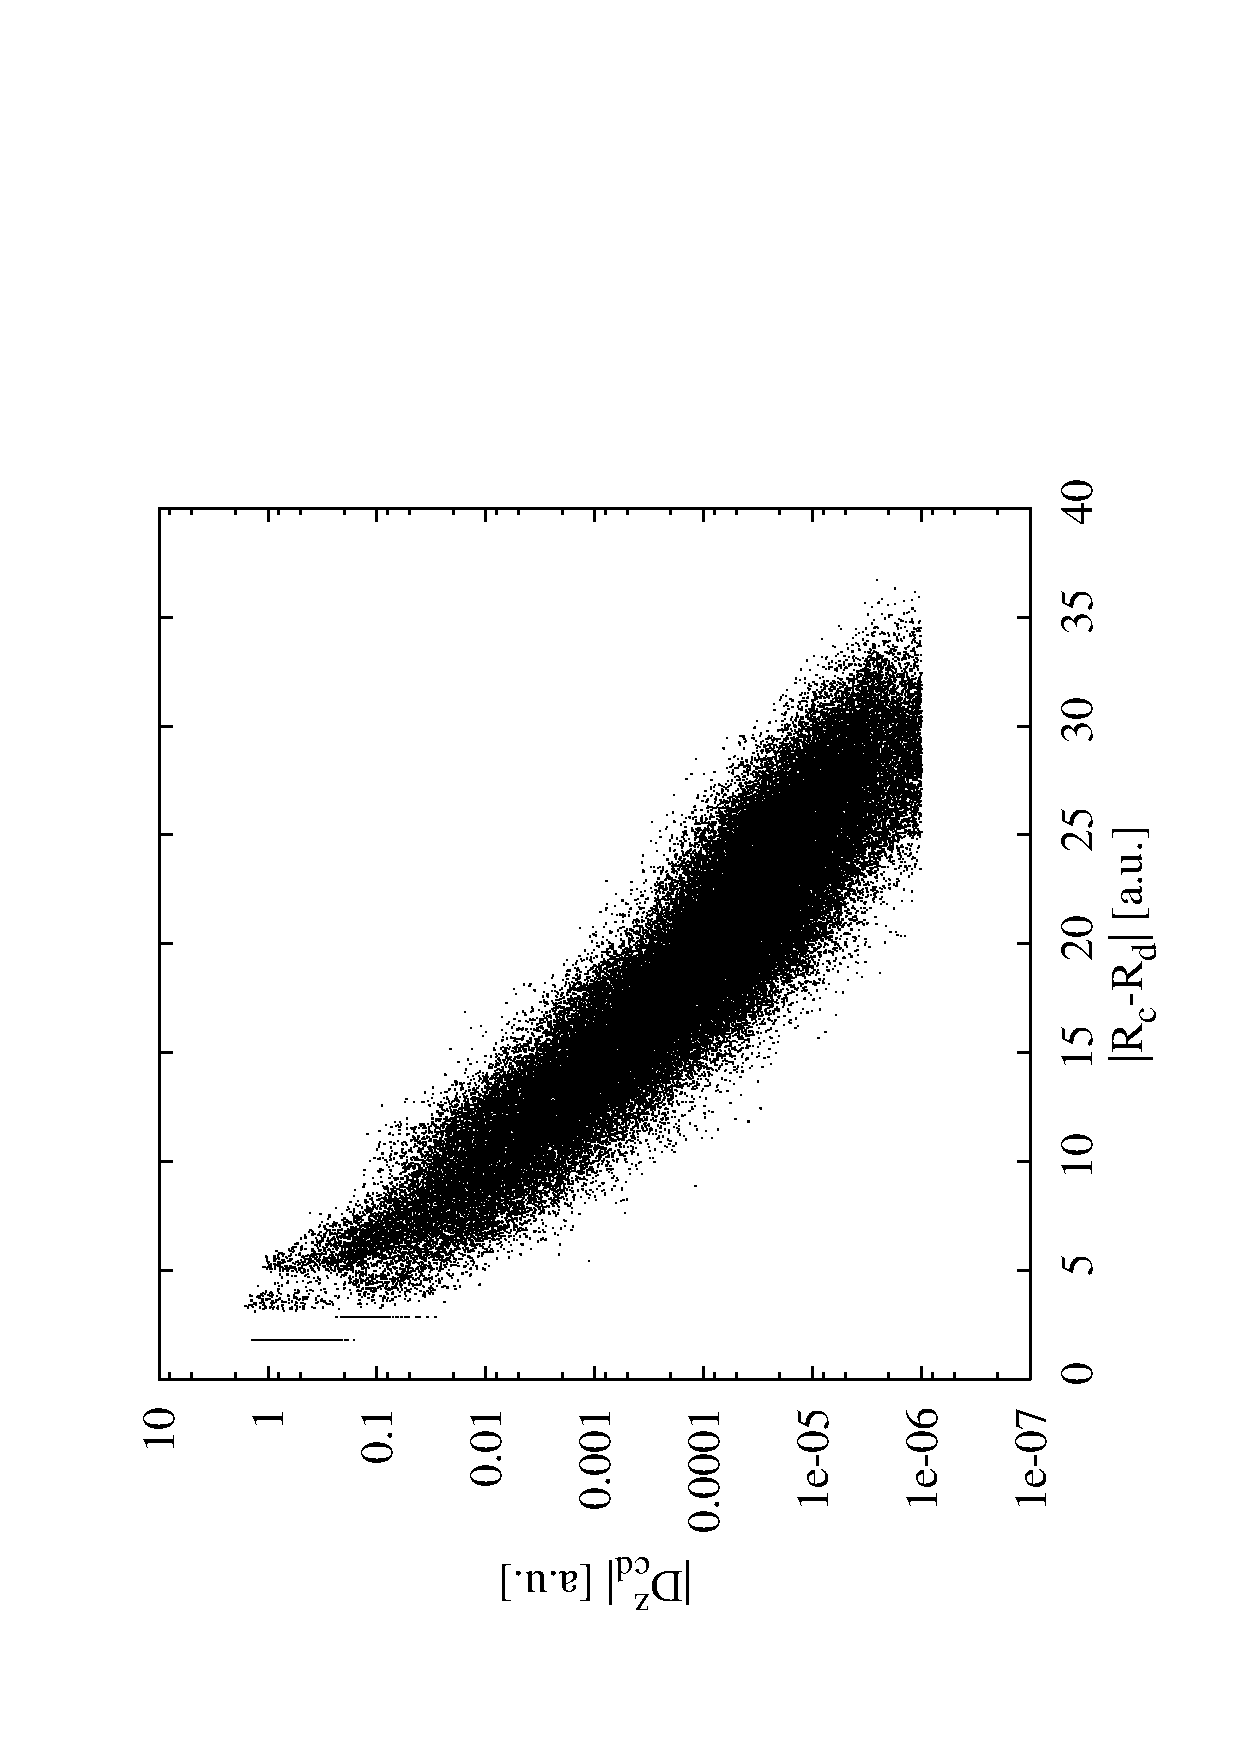
\includegraphics[angle=-90,width=0.5\textwidth]{DPrimeZ_150_6-31G}
  \end{center}
\end{figure}
%%%%%%%%%%%%%%%%%%%%%%%%%%%%%%%%%%%%%%%%%%%%%%%%%%%%%%%%%%%%%%%%
\begin{table}
  \centering
  \caption{\protect
    Average polarizability $\bar{\alpha}=(\alpha_{xx}+\alpha_{yy}+\alpha_{zz})/3N$
    for different water clusters with the 6-31G and 6-31G** basis sets
    with the $Good$ and $Tight$ accuracy (See text) and the results obtained with
    the GAMESS quantum chemistry package \cite{gamess} with the 6-31G. 
    All the results are in $[a.u.]$.
  }\label{tab:Polari_Values}
  \begin{ruledtabular}
    \begin{tabular}{cccccc}
      &\multicolumn{1}{c}{6-31G\footnotemark[1]}
      &\multicolumn{2}{c}{6-31G\footnotemark[2]}
      &\multicolumn{2}{c}{6-31G**\footnotemark[2]}\\
      $N$ & & $Good$ & $Tight$
          & $Good$ & $Tight$\\
      \hline
      10  & 4.569083 &  &  & 4.569102 & 5.479049  \\
      30  & 4.673213 &  &  & 4.673227 & 5.585280  \\
      50  & $-$      &  &  & 4.703568 & 5.622830  \\
      70  & $-$      &  &  & 4.732279 & 5.654747  \\
      90  & $-$      &  &  & 4.775024 & 5.695564  \\
      110 & $-$      &  &  & 4.780809 & 5.698447  \\
      130 & $-$      &  &  & 4.786437 & 5.704947  \\
      150 & $-$      &  &  & 4.775231 & 5.693447  \\
    \end{tabular}
  \end{ruledtabular}
 \footnotetext[1]{GAMESS calculations.}
 \footnotetext[2]{MondoSCF calculations.}
\end{table}
%%%%%%%%%%%%%%%%%%%%%%%%%%%%%%%%%%%%%%%%%%%%%%%%%%%%%%%%%%%%%%%%
%%%%%%%%%%%%%%%%%%%%%%%%%%%%%%%%%%%%%%%%%%%%%%%%%%%%%%%%%%%%%%%%
\section{Conclusion}


% We have presented a simple and efficient algorithm for the 
% computation of the response density matrix to an external 
% static electric field, we have also shown that the locality
% of the density matrix derivatives
% and an appropriate purification scheme can give rise to linear 
% scaling for the computation of the first electric polarizability.

% A self consistent first principle linear scaling 
% method for the calculation of the static electric
% polarizability was introduced. 



 We have presented a simple and efficient linear
 scaling algorithm for the self consistent
 calculation of the static electric polarizability.
 The locality of
 density matrix response was shown to hold also
 upon an global electric perturbation, with an
 exponential decay of the matrix element. This 
 shows that linear scaling self consistent 
 \emph{ab-inito} theory can be extended also to
 the computation of response properties. The
 accuracy and the efficiency of the linear scaling
 method was demonstrated for a series of water
 cluster.

 It was shown that the calculated polarizabilities
 were fairly insensitive to the numerical thresholds.
 This means that a considerable speed-up can be
 achived by using larger thresholds. The algorithm 
 described in Eq. (\ref{alg}) can be extended to 
 higher order response functions and to a 
 large class of molecular properties \cite{Me}.
 The method can be used to compute molecular
 properties such as for example the electric
 polarizabities, nuclear magnetic shielding 
 tensor (NMR shift), indirect spin-spin 
 coupling, electronic g-tensor and polarizability
 derivatives.


\subsection{future work: }



% We have presented a simple and efficient algorithm for the 
% computation of the response density matrix to an external 
% static electric field, we have also shown that the locality
% of the density matrix derivatives
% and an appropriate purification scheme can give rise to linear 
% scaling for the computation of the first electric polarizability.


% The density matrix derivative
% seems to follow an exponential decay as the ground state 
% density matrix for insulator systems. But as previously mentioned
% the higher the order of the response is, the less sparse the 
% response density matrix is. Higher order static and 
% time-dependent electric response functions are currently 
% under investigation.
%%%%%%%%%%%%%%%%%%%%%%%%%%%%%%%%%%%%%%%%%%%%%%%%%%%%%%%%%%%%%%%%
%%%%%%%%%%%%%%%%%%%%%%%%%%%%%%%%%%%%%%%%%%%%%%%%%%%%%%%%%%%%%%%%
%Acknowledgements
\begin{acknowledgments}
 This work has been supported by the US Department of Energy 
 under contract <NUMBER>.... The Advanced Computing Laboratory of Los 
 Alamos National Laboratory is acknowledged.
 All the numerical computations have been
 performed on computing resources located at this facility.
\end{acknowledgments}
%%%%%%%%%%%%%%%%%%%%%%%%%%%%%%%%%%%%%%%%%%%%%%%%%%%%%%%%%%%%%%%%
%%%%%%%%%%%%%%%%%%%%%%%%%%%%%%%%%%%%%%%%%%%%%%%%%%%%%%%%%%%%%%%%
\bibliography{Response2}
%%%%%%%%%%%%%%%%%%%%%%%%%%%%%%%%%%%%%%%%%%%%%%%%%%%%%%%%%%%%%%%%
%%%%%%%%%%%%%%%%%%%%%%%%%%%%%%%%%%%%%%%%%%%%%%%%%%%%%%%%%%%%%%%%
\begin{figure}
  \centering
  \caption{\protect
  Total CPU time of the fifth CPSCF iteration for the water
  cluster sequence with
  the 6-31G basis set and thresholds $Good$ and $Tight$ (See test).
  The lines are fits to the last four points.
  }\label{fig:Alpha_h2o3D_6-31G_G_T_t}
  \begin{center}
    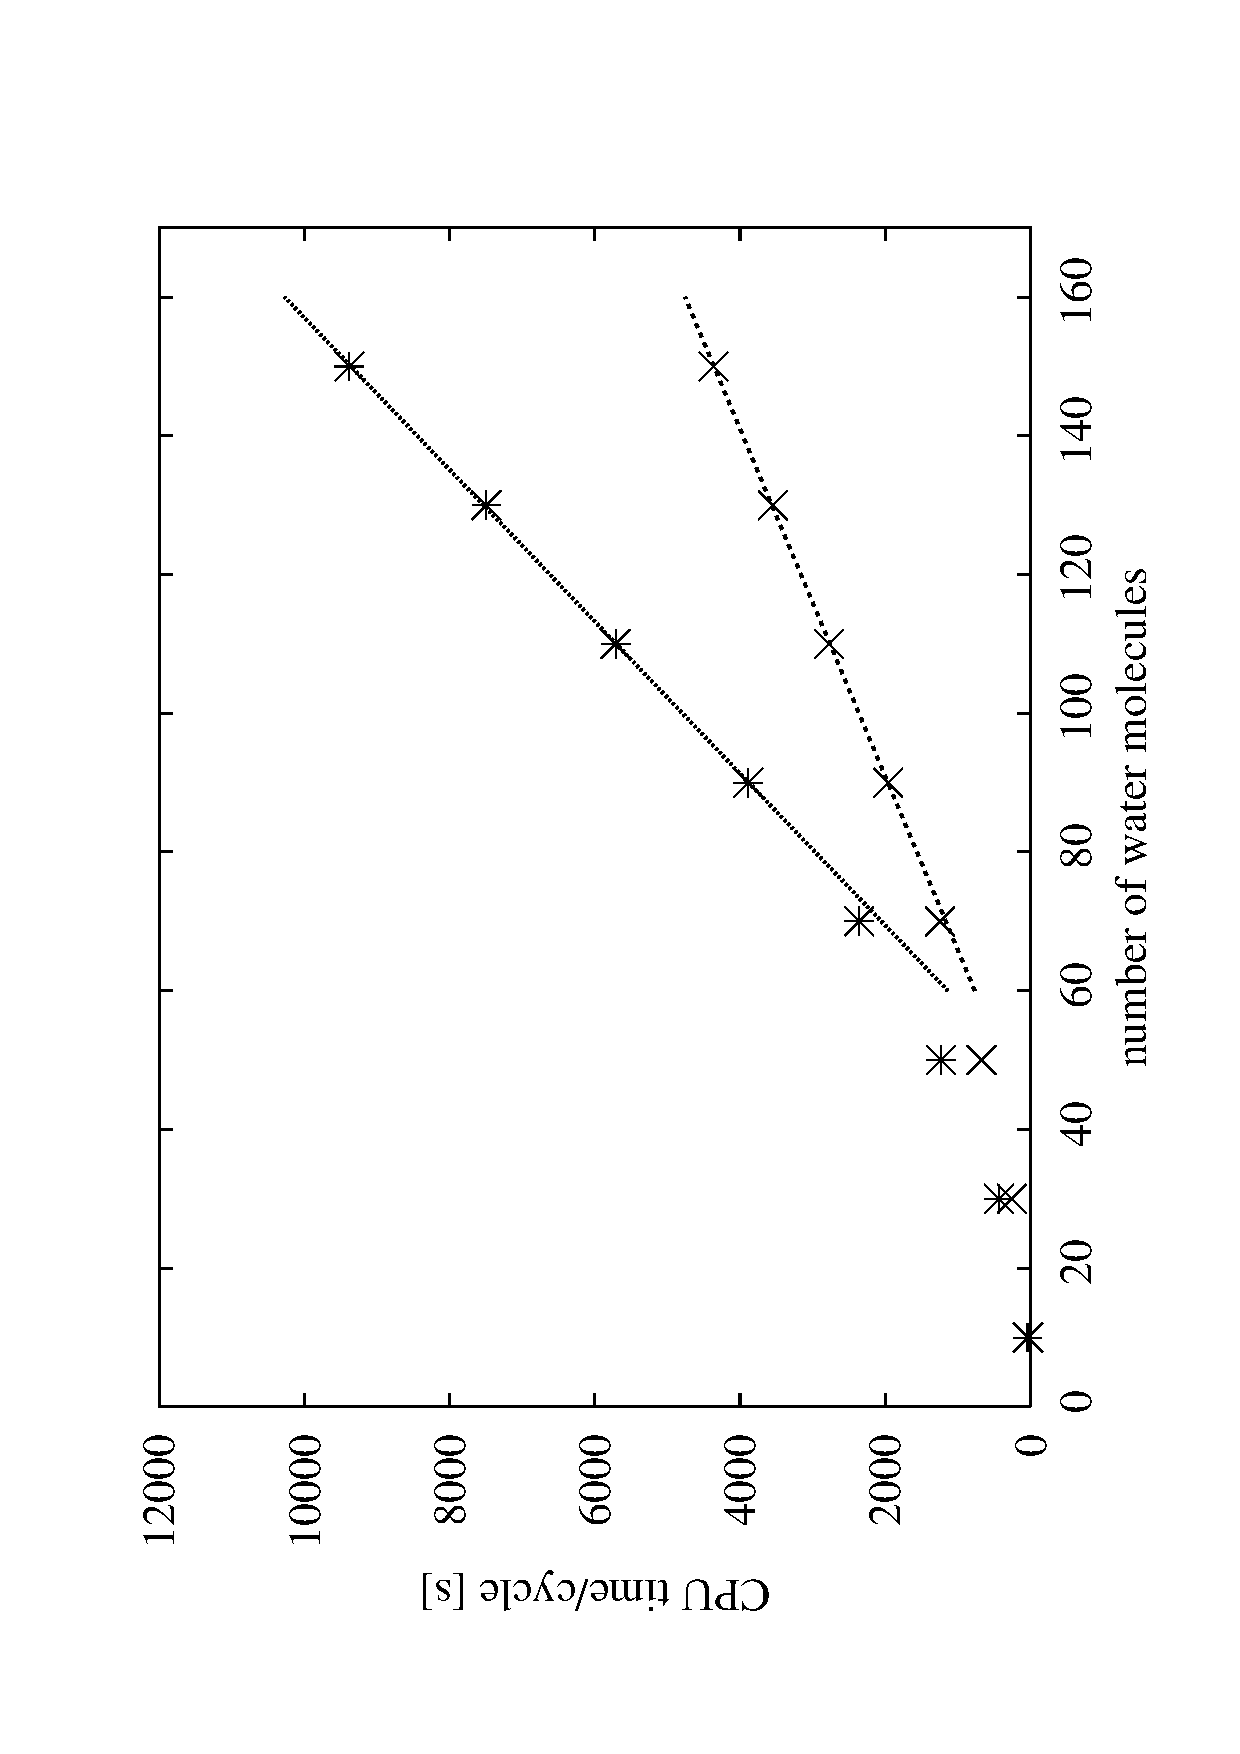
\includegraphics[angle=-90,width=0.5\textwidth]{Alpha_h2o3D_6-31G_G_T_t}
  \end{center}
\end{figure}
%%%%%%%%%%%%%%%%%%%%%%%%%%%%%%%%%%%%%%%%%%%%%%%%%%%%%%%%%%%%%%%%
\begin{figure}
  \centering
  \caption{\protect
  Total CPU time of the fifth CPSCF iteration for the water
  cluster sequence with
  the 6-31G** basis set and thresholds $Good$ and $Tight$ (See test).
  The lines are fits to the last three points.
  }\label{fig:Alpha_h2o3D_6-31Gss_G_T_t}
  \begin{center}
    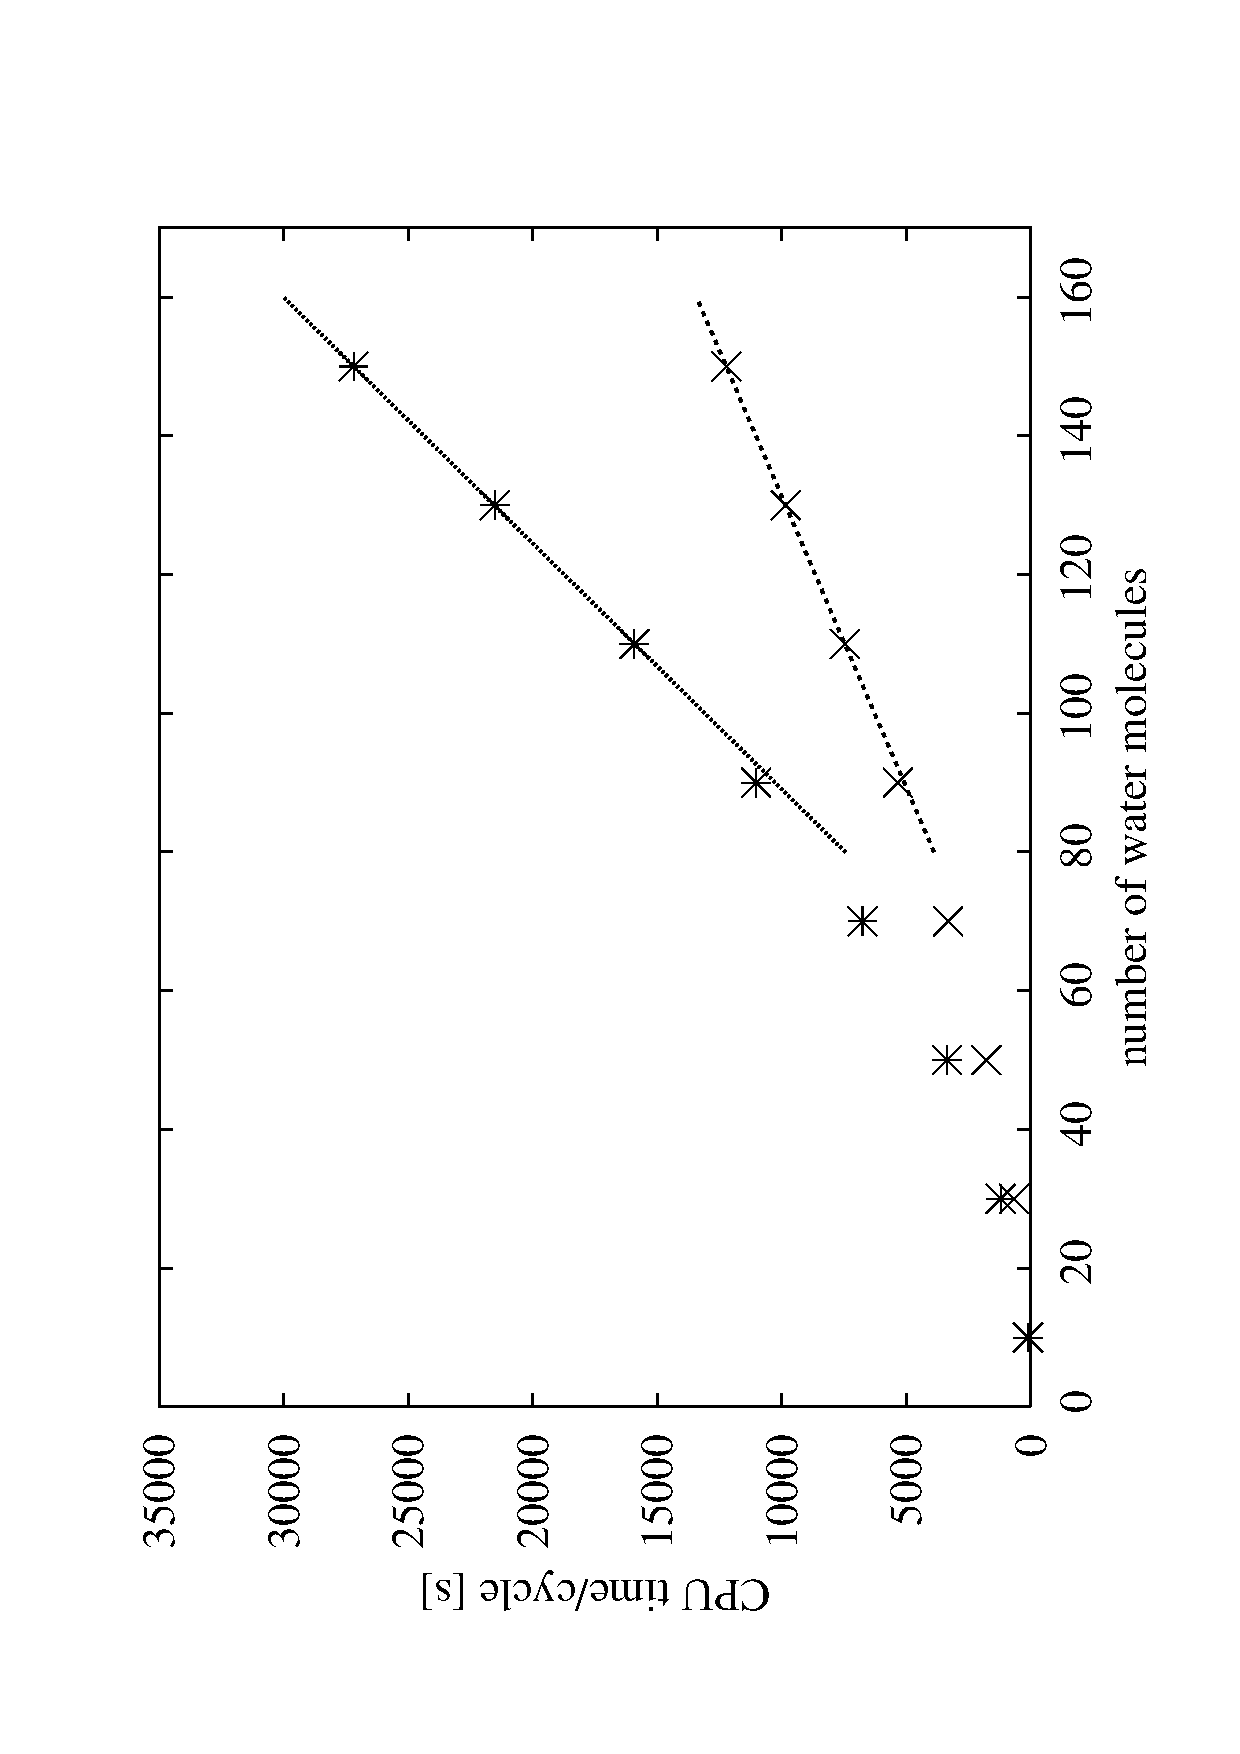
\includegraphics[angle=-90,width=0.5\textwidth]{Alpha_h2o3D_6-31Gss_G_T_t}
  \end{center}
\end{figure}

\end{document}
%
% ****** End of file apssamp.tex ******
